%%%%%%%%%%%%%%%%%%%%%%%%%%%%%%%%%%%%%%%%%%%%%%%%%%%%%%%%%%%%%%%%%%%%%%%%%%%%%%%%
\chapter{ТЕСТИРОВАНИЕ, АНАЛИЗ ПОЛУЧЕННЫХ РЕЗУЛЬТАТОВ}
%%%%%%%%%%%%%%%%%%%%%%%%%%%%%%%%%%%%%%%%%%%%%%%%%%%%%%%%%%%%%%%%%%%%%%%%%%%%%%%%

В данном разделе рассматривается тестовое окружение и ручное функциональное тестирование. Модульное тестирование не проводилось, потому что в коде в основном создавались обёртки над библиотекой sipML5, а эта библиотека протестирована создателями.

\section{Тестовое окружение}

Тестовое окружение серверной части было приведено в разделе \ref{section:config}.

Тестирование проводилось на браузерах Iceweasel 38.7.1, Mozilla Firefox 47.0, в них звонок работает хорошо. Также проводилось тестирование в браузерах Google Chrome 50.0.2661.75, Opera 38.0.2220.31, но на них не удалось полностью управлять звонком: иногда голос передавался только в одну сторону, иногда не удавалось его завершить. Однако следует заметить, что демо-версия sipML5 клиента\cite{sipML5_demo} работает на данных браузерах так же.

Из этого можно сделать вывод, Google Chrome ведёт себя так из-за нововведения в версии 47, которое запрещает функцию getUserMedia() если используется протокол HTTP, и позволяет её только для протокола HTTPS.\cite{chrome_https} Почему демо-версия sipML5 работает со сбоями в браузере Opera пока не ясно.

\section{Функциональное тестирование}

Автоматизированного функционального тестирования не проводилось из-за трудоёмкости задачи. У Asterisk имеются встроенные средства записывать звонки. При таком тестировании необходимо было бы реализовать тестовый модуль SIP-телефонии, который бы записывал во время звонка две дорожки - одну с микрофона, другую поступающую от собеседника. Помимо этого, необходимо было бы создать тестовые сценарии, которые можно сделать например в Selenium IDE. После выполнения этих сценариев, необходимо отправить файлы записи звонка от Asterisk клиенту и сравнить их с файлами записанными тестовым модулем SIP-телефонии.

Поэтому функциональное тестирование проводилось вручную.

Критерии корректной работы модуля SIP-телефонии:
\begin{itemize}
\item Аутентификация и деаутентификация на сервере.
\item Сессия аутентификации должна корректно переходить из одного состояния в другое.
\item Корректные инициализация вызова и воспроизведение рингтона и гудков.
\item Сессия звонка должна корректно переходить из одного состояния в другое.
\item При звонке передача голоса должна быть в обе стороны.
\item В графическом интерфейсе в определённые состояния звонка должны быть неактивны определённые кнопки. Например, в момент разговора кнопка звонка должна быть выключена и доступна только кнопка сброса.
\item Корректная обработка звонков на несуществующие номера.
\end{itemize}

Проверялись инициализация вызова как входящего, так и исходящего. Проверялось завершение вызова, инициируемое как нашим клиентом, так и клиентом собеседника. Завершение вызова проверялось как в момент разговора, так и в момент до снятия трубки. Так же отслеживался лог-звонка на сервере Asterisk. Полностью прошёл все тестовые сценарии только SIP-модуль, запущенный в браузере Firefox. В его логе звонка ошибок не было (см. листинг \ref{listings:call}).

\lstinputlisting[
label={listings:call},
caption={Лог звонка на сервере Asterisk, 103 - реализованный SIP-модуль, 101 - SIP-клиент на мобильном устройстве CSipSimple},
]
{src/call.log}

На рисунках \ref{image:test1} - \ref{image:test8} изображён корректный графический интерфейс модуля в разных состояниях. Описание состояния читайте в названиях рисунков.

На рисунке \ref{image:test1} видно кнопку "телефон". Это скользящая кнопка, выполняет функцию скрытия и отображения плавающего окна.

\begin{figure}[h!]
\center{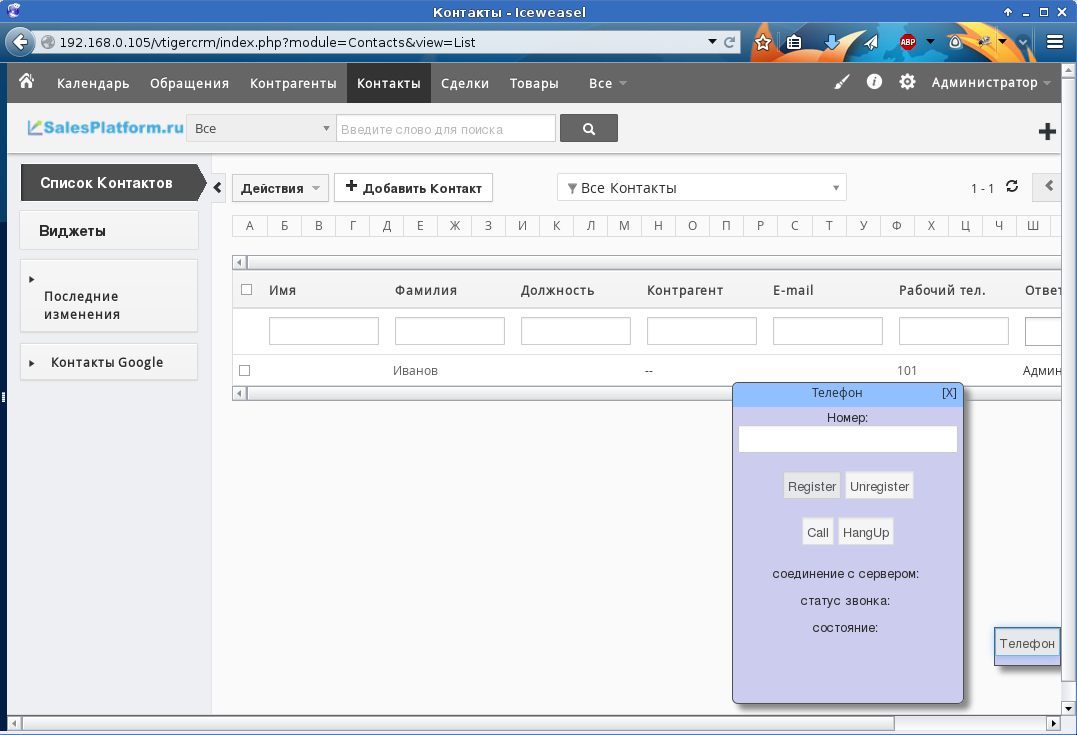
\includegraphics[width=0.75\linewidth]{test1}}
\caption{Модуль в CRM-системе SalesPlatform vtiger CRM 6.4, начальное состояние модуля}
\label{image:test1}
\end{figure}

\begin{figure}[h]
\center{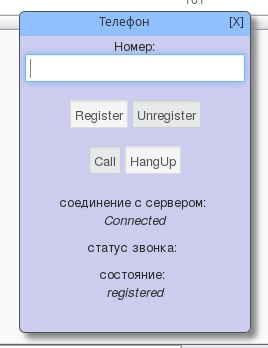
\includegraphics[width=0.4\linewidth]{test2}}
\caption{Состояние после аутентификации на сервере}
\label{image:test2}
\end{figure}

\begin{figure}[h]
\center{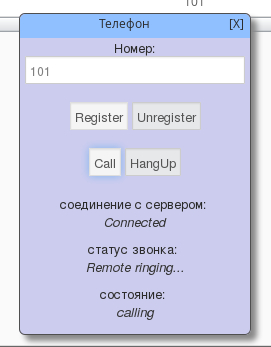
\includegraphics[width=0.4\linewidth]{test3}}
\caption{Состояние исходящего звонка (воспроизводятся гудки)}
\label{image:test3}
\end{figure}

\begin{figure}[h]
\center{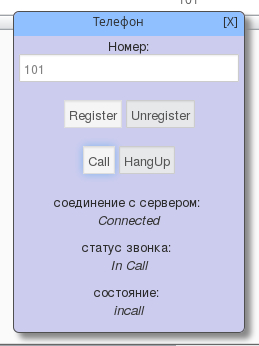
\includegraphics[width=0.4\linewidth]{test4}}
\caption{Состояние в процессе звонка}
\label{image:test4}
\end{figure}

\begin{figure}[h]
\center{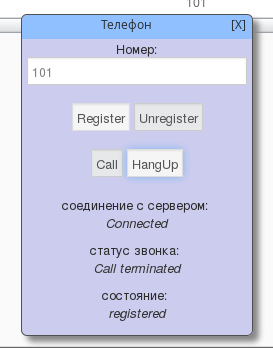
\includegraphics[width=0.4\linewidth]{test5}}
\caption{Состояние завершения звонка, такое же как и состояние после аутентификации на сервере}
\label{image:test5}
\end{figure}

\begin{figure}[h]
\center{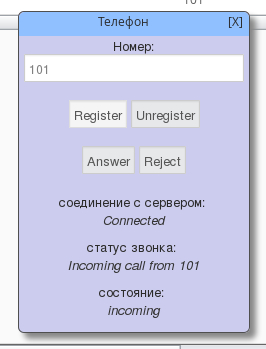
\includegraphics[width=0.4\linewidth]{test6}}
\caption{Состояние входящего звонка (воспроизводится рингтон)}
\label{image:test6}
\end{figure}

\begin{figure}[h]
\center{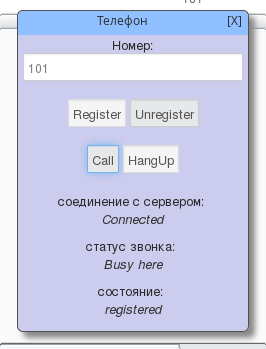
\includegraphics[width=0.4\linewidth]{test7}}
\caption{Вызываемый абонент занят}
\label{image:test7}
\end{figure}

\begin{figure}[h]
\center{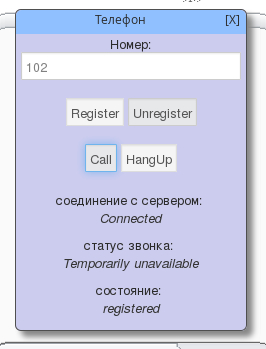
\includegraphics[width=0.4\linewidth]{test8}}
\caption{Вызываемый абонент недоступен}
\label{image:test8}
\end{figure}

\section{Анализ полученных результатов}

В итоге имеем реализацию модуля SIP-телефонии для web-браузера. В нём осуществляется контроль за состоянием звонка. Модуль фоново работает на странице. Данный модуль разработан так, чтобы мог встраиваться в любые бизнес-системы и CRM-системы.

Модуль был частично встроен в vtiger CRM. Реализован click-to-call. Не реализована часть, получающая информацию о SIP-аккаунте пользователя. Также не реализована часть, которая управляет карточкой звонка.

Модуль пока что работает в браузере Firefox и частично в Chrome и Opera.

\section{Резюме}

Описано тестовое окружение. Проведено функциональное тестирование. По ходу разработки, оно помогало выявить следующие функциональные ошибки: некорректное состояние сессии звонка, односторонняя передача голоса и некорректное состояние графического интерфейса. Проведён анализ полученных результатов.
